\documentclass[english,letter paper,12pt,leqno]{article}
\usepackage{array}
\usepackage{stmaryrd}
\usepackage{amsmath, amscd, amssymb, mathrsfs, accents, amsfonts,amsthm}
\usepackage[all]{xy}
\usepackage{dsfont}
\usepackage{tikz}
\def\nicedashedcolourscheme{\shadedraw[top color=blue!22, bottom color=blue!22, draw=gray, dashed]}
\def\nicecolourscheme{\shadedraw[top color=blue!22, bottom color=blue!22, draw=white]}
\def\nicepalecolourscheme{\shadedraw[top color=blue!12, bottom color=blue!12, draw=white]}
\def\nicenocolourscheme{\shadedraw[top color=gray!2, bottom color=gray!25, draw=white]}
\def\nicereallynocolourscheme{\shadedraw[top color=white!2, bottom color=white!25, draw=white]}
\definecolor{Myblue}{rgb}{0,0,0.6}
\usepackage[a4paper,colorlinks,citecolor=Myblue,linkcolor=Myblue,urlcolor=Myblue,pdfpagemode=None]{hyperref}

\SelectTips{cm}{}

\setlength{\evensidemargin}{0.1in}
\setlength{\oddsidemargin}{0.1in}
\setlength{\textwidth}{6.3in}
\setlength{\topmargin}{0.0in}
\setlength{\textheight}{8.5in}
\setlength{\headheight}{0in}

\newtheorem{theorem}{Theorem}[section]
\newtheorem{proposition}[theorem]{Proposition}
\newtheorem{lemma}[theorem]{Lemma}
\newtheorem{corollary}[theorem]{Corollary}
\newtheorem{setup}[theorem]{Setup}

% Labels in tabular
\newcommand{\tagarray}{\mbox{}\refstepcounter{equation}$(\theequation)$}

\newtheoremstyle{example}{\topsep}{\topsep}
	{}
	{}
	{\bfseries}
	{.}
	{2pt}
	{\thmname{#1}\thmnumber{ #2}\thmnote{ #3}}
	
	\theoremstyle{example}
	\newtheorem{definition}[theorem]{Definition}
	\newtheorem{example}[theorem]{Example}
	\newtheorem{remark}[theorem]{Remark}
	\newtheorem{strat}[theorem]{Strategy}

\numberwithin{equation}{section}

% Operators
\def\eval{\operatorname{ev}}
\def\res{\operatorname{Res}}
\def\Coker{\operatorname{Coker}}
\def\Ker{\operatorname{Ker}}
\def\im{\operatorname{Im}}
\def\can{\operatorname{can}}
\def\K{\mathbf{K}}
\def\D{\mathbf{D}}
\def\N{\mathbf{N}}
\def\LG{\mathcal{LG}}
\def\Ab{\operatorname{Ab}}
\def\stab{\operatorname{stab}}
\def\Hom{\operatorname{Hom}}
\def\modd{\operatorname{mod}}
\def\Modd{\operatorname{Mod}}
\def\be{\begin{equation}}
\def\ee{\end{equation}}
\def\nN{\mathds{N}}
\def\nZ{\mathds{Z}}
\def\nQ{\mathds{Q}}
\def\nR{\mathds{R}}
\def\nC{\mathds{C}}
\DeclareMathOperator{\Ext}{Ext}
\DeclareMathOperator{\Tr}{Tr}
\DeclareMathOperator{\End}{End}
\DeclareMathOperator{\rank}{rank}
\DeclareMathOperator{\tot}{Tot}
\DeclareMathOperator{\ch}{ch}
\DeclareMathOperator{\str}{str}
\DeclareMathOperator{\hmf}{hmf}
\DeclareMathOperator{\HMF}{HMF}
\DeclareMathOperator{\hf}{HF}
\DeclareMathOperator{\At}{At}
\DeclareMathOperator{\Cat}{Cat}
\DeclareMathOperator{\Spec}{Spec}
\DeclareMathOperator{\id}{id}

\begin{document}

% Commands
\def\Res{\res\!}
\newcommand{\ud}{\mathrm{d}}
\newcommand{\Ress}[1]{\res_{#1}\!}
\newcommand{\cat}[1]{\mathcal{#1}}
\newcommand{\lto}{\longrightarrow}
\newcommand{\xlto}[1]{\stackrel{#1}\lto}
\newcommand{\mf}[1]{\mathfrak{#1}}
\newcommand{\md}[1]{\mathscr{#1}}
\def\sus{\l}
\def\l{\,|\,}
\def\sgn{\textup{sgn}}

\title{$A_\infty$-minimal models of matrix factorisations}
\author{Daniel Murfet}

\maketitle

\begin{abstract}
We study $A_\infty$-minimal models of the differential graded algebras obtained from endomorphisms of generators of triangulated categories of matrix factorisations, giving explicit higher products for the cases of simple singularities. 
\end{abstract}

\section{Introduction}

Let $k$ be a commutative $\mathbb{Q}$-algebra and $W \in k[x_1,\ldots,x_n]$ a polynomial which is a potential over $k$ in the sense of \cite[\S 2.2]{lgdual}. For example, $k = \mathbb{C}$ and $W$ has isolated critical points. The $\nZ_2$-graded DG-category $\cat{A} = \operatorname{mf}(R, W)$ has for its objects finite-rank matrix factorisations of $W$ over $R = k[x_1,\ldots,x_n]$. In this paper we study the minimal model problem for $\cat{A}$, the aim being to produce models that are finitely-generated and projective over $k$.

When $k$ is a field, the standard minimal model theorem \cite{??} constructs the structure of an $A_\infty$-category on the cohomology $\cat{B} = H^* \cat{A}$ in such a way that $\cat{B}$ is quasi-isomorphic to $\cat{A}$. Moreover, this $A_\infty$-category has finite-dimensional Hom-spaces and is therefore a good finite model of $\cat{A}$. The problem in this case is to have sufficient control over the inputs to the minimal model theorem that the $A_\infty$-products on $H^* \cat{A}(X,X)$ can be reasonably calculated, for a given matrix factorisation $X$. In order to understand deformations of matrix factorisations \cite{??,??,??} it is important to do this for generic $X$, but the special case where $X = k^{\stab}$, the generator of $\cat{A}$ studied by Dyckerhoff in the case of a single isolated singularity at the origin \cite{d0904.4713}, is of particular interest.

Since one of our goals is to understand how matrix factorisation categories vary along unfoldings of singularities, we also need to consider the case where $k$ is not a field. For example take $k = \mathbb{C}[t]$ and $R = \mathbb{C}[x_1,\ldots,x_n, t]$ so that $W = W_t(x)$ is a potential with parameter. In this case we want an $A_\infty$-category $\cat{B}$ quasi-isomorphic to $\cat{A}$ over $k$, with $\cat{B}(a,b)$ a finitely-generated projective $k$-module for each pair of objects $a,b$. 
\vspace{0.2cm}

These two desiderata, understanding the $A_\infty$-products on $H^*\cat{A}(X,X)$ for generic $X$, and the case where $k$ is not a field, lead us naturally to a slightly non-standard use of the minimal model theorem. Following the ideas developed in \cite{??,??,??} we prove that, writing $\iota: R \lto R/(\partial_{x_1} W, \ldots, \partial_{x_n} W)$ for the quotient, there is a $k$-linear homotopy retract
\be\label{eq:intro_he}
\xymatrix@C+4pc{
\iota^* \cat{A} \ar@<0.7ex>[r] & \cat{A} \otimes_k \bigwedge\big( k^{\oplus n}[1] \big) \ar@<0.7ex>[l]\,.
}
\ee

Suppose $W \in \mf{m}^2$ where $\mf{m} = (x_1,\ldots,x_n)$ and choose a presentation $W = x_1 W^1 + \cdots + x_n W^n$ with $W^i \in \mf{m}$ and consider the following pair
\begin{equation}\label{eq:kstab}
k^{\operatorname{stab}} = \Big( k[x] \otimes_k \bigwedge( k\psi_1 \oplus \cdots \oplus k \psi_n ), \;d_{k^{\stab}} = \sum_{i=1}^n x_i \psi_i^* + \sum_{i=1}^n W^i \psi_i \Big)
\end{equation}
where $\psi_i^*$ and $\psi_i$ act respectively by contraction and wedge product on the exterior algebra underlying $k^{\stab}$. It is easy to see that $d_{k^{\stab}}^2 = W$, so $k^{\stab}$ is a matrix factorisation. When $k$ is a field and $W$ has an isolated critical point at the origin, $k^{\stab}$ is the representative in the homotopy category of matrix factorisations of the structure sheaf of the singular point at the origin, and was first studied by Dyckerhoff \cite{d0904.4713}. 

The purpose of this paper is to show how to calculate the $A_\infty$-minimal model of the $\nZ_2$-graded differential graded endomorphism algebra of this matrix factorisation
\be\label{eq:defnaw}
\Big( \End_{k[x]}(k^{\operatorname{stab}}), \; \partial = [d_{k^{\stab}},-] \; \Big)\,.
\ee 
The differential here is (throughout all commutators are graded commutators)
\begin{align*}
\partial = [d_{k^{\stab}},-] &= \Big[\sum_i x_i \psi_i^* + \sum_i W^i \psi_i, -\Big]\\
&= \sum_i x_i [\psi_i^*,-] + \sum_i W^i [\psi_i,-]\,.
\end{align*}
The minimal model is a finite-dimensional $\nZ_2$-graded vector space $\md{M}_W$ with a family 
\[
\left\{ r_q: \big(\md{M}_W[1]\big)^{\otimes q} \lto \md{M}_W[1] \right\}_{q \ge 2}
\]
of odd $k$-linear maps satisfying the forward suspended $A_\infty$-constraints \cite{lazaroiu}, and having the property that there is an $A_\infty$-quasi-isomorphism $\md{M}_W \lto \End_{k[x]}(k^{\stab})$.

\section{Background}

\subsection{A-infinity algebras}

The \emph{tilde grading} is defined by $\widetilde{x} = |x| - 1$.

Throughout $\otimes = \otimes_k$.

\section{Perturbation and Koszul complexes}

Let $k$ be a characteristic zero field, $R =  k[x_1,\ldots,x_n]$ and let $W \in \mf{m}^2$ be a potential with chosen decomposition $W = \sum_{i=1}^n x_i W^i$. To apply the $A_\infty$-minimal model construction to the DG-algebra $\md{A}_W$ from \eqref{eq:defnaw} we would usually begin by finding a $k$-linear homotopy retract of this complex onto its cohomology. However, for our purposes it is better to first enlarge the DG-algebra to $S \otimes \md{A}_W$, where $S$ is the $\nZ_2$-graded vector space
\be
S = \bigwedge( k\theta_1 \oplus \cdots \oplus k \theta_n )
\ee
with grading $|\theta_i| = 1$. We make the tensor product $S \otimes \md{A}_W$ into a DG-algebra in the usual way, giving the exterior algebra $S$ the zero differential.

\begin{definition} We define the finite-dimensional $\nZ_2$-graded vector space
\be\label{eq:defnunderlineend}
\md{E} = R/\mf{m} \otimes \End_R(k^{\stab}) \cong \End_k\Big( \bigwedge( k\psi_1 \oplus \cdots \oplus k \psi_n) \Big)
\ee
where $\mf{m} = (x_1,\ldots,x_n)$.
\end{definition}

We will show that $S \otimes \md{A}_W$ is homotopy equivalent to $\md{E}$ viewed as a complex with zero differential (observe that $\md{E}$ does not depend on $W$). The corresponding homotopy retract (see Proposition \ref{prop:he_start} below) is our starting point for the minimal model construction. For this we use the Koszul complex of $x_1,\ldots,x_n$,
\be\label{eq:defnkoszulK}
K = \Big( R \otimes \bigwedge( k\theta_1 \oplus \cdots \oplus k \theta_n ), \; d_K = \sum_i x_i \theta_i^*\; \Big)
\ee

\begin{theorem} There is a diagram of $\nZ_2$-graded complexes and homotopy equivalences over $k$
\be\label{eq:first_he}
\xymatrix@C+3pc{
S \otimes \md{A}_W \ar@<1ex>[r]^-{\exp(-\delta)} & K \otimes_R \md{A}_W \ar@<1ex>[l]^-{ \exp(-\delta) } \ar@<1ex>[r]^-{\pi} & \md{E}\,.\ar@<1ex>[l]^-{ \sigma_\infty }
}
\ee
\end{theorem}
\begin{proof}
See \cite{murfet}.
\end{proof}

The notation is as follows:
\begin{itemize}
\item The complexes involved here are
\begin{gather*}
\big( S \otimes \End_R(k^{\stab}), \; \partial \,\big)\\
\big( K \otimes_R \End_R(k^{\stab}), \; d_K + \partial\, \big)\\
\big( \md{E}, 0 \big)\,.
\end{gather*}
\item The operator $\psi_j = \psi_j \wedge -$ on $k^{\stab}$ satisfies
\[
[ \psi_j, d_{k^{\stab}} ] = \big[ \psi_j, \sum_i x_i \psi_i^* \big] = x_j \cdot 1\,,
\]
where $[-,-]$ always denotes the graded commutator. That is, $\psi_j$ is a homotopy for the action of $x_j$ on $k^{\stab}$. It is then easy to check that the odd operator $\alpha \mapsto \psi_j \circ \alpha$ on $\End_R(k^{\stab})$ is also a homotopy for $x_j$, and where it will not cause confusion we will also write $\psi_j$ for this operator of post-composition.

\item Both $S \otimes \md{A}_W$ and $K \otimes_R \md{A}_W$ have the same underlying $\nZ_2$-graded $k$-module, namely
\be\label{eq:same_underlying}
R \otimes \bigwedge( k\theta_1 \oplus \cdots \oplus k \theta_n ) \otimes \End_k\big( \bigwedge( k\psi_1 \oplus \cdots \oplus k \psi_n ) \big)\,.
\ee
On this space we define the even operator
\be
\delta = \sum_{i=1}^n \psi_i \theta_i^*\,,
\ee
where $\psi_i$ is the operator on $\End_R(k^{\stab})$ discussed above, given by $\alpha \mapsto (\psi_i \wedge -) \circ \alpha$, and $\theta_i^*$ acts by contraction on $S$. It is easy to check that $\exp(\delta),\exp(-\delta)$ intertwines the differentials $\partial$ and $d_K + \partial$ and therefore gives an isomorphism between the first two complexes in \eqref{eq:first_he} \cite[Proposition 4.11]{murfet}.
\item The morphism of complexes $\pi: K \lto R/\mf{m}$ is defined by composing the projection of $K$ onto the submodule $R \cdot 1$ of $\theta$-degree zero forms, with the quotient $R \lto R/\mf{m}$. We also write $\pi$ for the result of tensoring this morphism with $\End_R(k^{\stab})$ to obtain
\[
\xymatrix@C+2pc{
K \otimes_R \End_R(k^{\stab}) \ar[r]^-{\pi \otimes 1} & R/\mf{m} \otimes_R \End_R(k^{\stab}) = \underline{\End}(k^{\stab})\,.
}
\]
This is a morphism of complexes, because the differential on $\End_R(k^{\stab})$ vanishes on the quotient $\underline{\End}(k^{\stab})$ by the hypothesis that $W \in \mf{m}^2$.
\item The $k$-linear homotopy inverse $\sigma_\infty$ to $\pi$ in \eqref{eq:first_he} is defined in terms of the following ingredients. The first is the $k$-linear connection (viewing $\theta_i$ as a $1$-form)
\be
\Delta: K \lto K\,, \qquad \Delta = \sum_i \partial_{x_i} \theta_i
\ee
and the degree $-1$ (with respect to the $\theta$-degree) $k$-linear operator
\be
H = [d_K, \Delta]^{-1} \Delta\,.
\ee
We write $\partial$ for the differential on $\End_R(k^{\stab})$, and $\sigma: k \lto K$ for the map which sends $\lambda \in k$ to $\lambda \cdot 1 \in K$, and define $k$-linear maps
\begin{align}
\sigma_\infty = \sum_{m \ge 0} (-1)^m (H \partial)^m \sigma\,,\\
H_\infty = \sum_{m \ge 0} (-1)^m (H \partial)^m H\,.
\end{align}
Here $H_\infty$ is an odd operator on $K \otimes_R \End_R(k^{\stab})$. These maps satisfy:
\begin{align}
\pi \sigma_\infty &= 1\,,\\
 \sigma_\infty \pi &= 1 - [d_K + \partial, H_\infty]\,.
\end{align}
\end{itemize}

By inspection of \eqref{eq:first_he}, we therefore have the following:

\begin{proposition}\label{prop:he_start} There is a diagram of morphisms of $\nZ_2$-graded $k$-complexes
\be\label{eq:he_start}
\xymatrix@C+5pc{
S \otimes \md{A}_W \ar@<1ex>[r]^-{\Phi} & \md{E}\ar@<1ex>[l]^-{\Phi^{-1}}
}
\ee
where $\Phi = \pi \exp(-\delta), \Phi^{-1} = \exp(\delta) \sigma_\infty$ and $\widehat{H} = \exp(\delta) H_\infty \exp(-\delta)$ satisfy
\be
\Phi \Phi^{-1} = 1\,, \qquad \Phi^{-1} \Phi = 1 - [\partial, \widehat{H}]\,.
\ee
Thus, $\Phi$ and $\Phi^{-1}$ are mutually inverse homotopy equivalences over $k$.
\end{proposition}

The endomorphism algebra $C = \End_k(S)$ is a Clifford algebra generated by the contraction $\theta_i^*$ and wedge product $\theta_i$ operators. It is observed in \cite{murfet} that \eqref{eq:he_start} is an isomorphism of Clifford representations (in the homotopy category) when the complex $\md{E}$ is equipped with the action induced by Atiyah classes:

\begin{definition}
The Atiyah classes of $\md{A}_W$ are the $R$-linear odd operators
\[
\At_i = [\partial, \partial_{x_i}]: \End_R(k^{\stab}) \lto \End_R(k^{\stab})\,,
\]
\end{definition}

\begin{lemma} We have
\[
\At_i = -[\psi_i^*, -] - \sum_{q=1}^n \partial_{x_i}(W^q) [ \psi_q, - ]\,.
\]
\end{lemma}
\begin{proof}
By direct calculation:
\begin{align*}
\At_i &= \big[ [d_{k^{\stab}},-], \partial_{x_i} \big]\\
&= \sum_q \big[x_q [\psi_q^*,-], \partial_{x_i}\big] + \sum_q \big[W^q [\psi_q,-], \partial_{x_i}\big]\\
&= -\sum_q \partial_{x_i}(x_q) [\psi_q^*,-] - \sum_q \partial_{x_i}(W^q) [\psi_q,-]\\
&= -[\psi_i^*,-] - \sum_q \partial_{x_i}(W^q) [\psi_q, -]\,.
\end{align*}
\end{proof}

\section{Trees and decorations}

\begin{example}
\end{example}

\section{Feynman diagrams}
% from p.17 (ainfmf9)

The integer $n$ is the number of variables in the ambient ring $R = k[x_1,\ldots,x_n]$. 

\begin{definition} Consider the $\nZ_2$-graded algebra defined by the tensor product
\[
\mathscr{H} = R \otimes_k \bigwedge\big( \oplus_{i=1}^n k \theta_i \,\big) \otimes_k \End_k\Big( \bigwedge\big( \oplus_{i=1}^n k \psi_i \, \big) \Big)
\]
with degrees $|\theta_i| = |\psi_i| = 1$. On this space we have the homogeneous operators
\[
x_i\,, \partial_i = \partial_{x_i}\,, \theta_i\,, \theta_i^*\,, \big[\psi_i\,,-\big]\,.
\]
Here $\psi_i$ denotes the operator $\psi_i \wedge (-)$ on $\bigwedge\big( \oplus_{i=1}^n k \psi_i \, \big)$ and $[ \psi_i, - ]$ the graded commutator with this operator, defined on a homogeneous operator $\beta$ by
\[
\big[ \psi_i, \beta \big] = \psi_i \circ \beta - (-1)^{|\beta|} \beta \circ \psi_i\,.
\]
We define the $\nZ_2$-graded $k$-module
\[
\mathscr{B} = \bigwedge\big( \oplus_{i=1}^n k \psi_i^* \,\big)
\]
which we view as a submodule
\[
\mathscr{B} \subset \End_k\Big( \bigwedge\big( \oplus_{i=1}^n k \psi_i \, \big) \Big)
\]
by identifying $\psi_i^* \in \mathscr{B}$ with the operation of contraction $\psi_i^*\, \lrcorner\, (-)$ on the exterior algebra. In this way we may also identify $\mathscr{B}$ with a submodule of $\mathscr{H}$, and we write $\iota: \mathscr{B} \lto \mathscr{H}$ for the inclusion. Note that the operator $[\psi_j, -]$ on $\mathscr{H}$ defined above acts on the submodule $\mathscr{B}$ as contraction with $\psi_j = (\psi_j^*)^*$, that is,
\be\label{eq:comm_is_ann}
\Big[ \psi_j, \iota\big(\psi_{i_1}^* \wedge \cdots \wedge \psi_{i_r}^*\big) \Big] = \sum_{l=1}^r (-1)^{l-1} \delta_{j, i_l} \iota\big(\psi_{i_1}^* \wedge \cdots \wedge \widehat{ \psi_{i_l}^* } \wedge \cdots \wedge \psi_{i_r}^*\big)\,.
\ee
We write $p: \mathscr{H} \lto \mathscr{B}$ for the natural projection (todo).
\end{definition}

We view $\mathscr{H}$ as the tensor product of the bosonic Fock space $R$ with creation and annihilation operators $x_i, \partial_i$, fermionic Fock space $\wedge( \oplus_{i=1}^n k \theta_i )$ with creation and annihilation operators $\theta_i, \theta_i^*$ and the third factor, of which the calculations of the $A_\infty$-structure only involve the submodule $\mathscr{B} = \wedge( \oplus_{i=1}^n k \psi_i^* )$ which is another fermionic Fock space. The inputs to the Feynman diagrams are tensor products of states in $\mathscr{B}$, that is, wedge products of $\psi_i^*$'s, on which the $[\psi_i, -]$ act as annihilation operators.

The linear maps in \eqref{eq:int_input}, \eqref{eq:int_intedge}, \eqref{eq:int_intvert} below which determine the $A_\infty$ products $\rho_q$ on $\mathscr{B}$ will be defined in terms of these creation and annihilation operators on $\mathscr{H}$, and may be interpreted as particle interactions in the usual way. The interactions that appear are the following ones, depicted on the left as Feynman diagrams and on the right as operators. We call these respectively \emph{A-, B- and C-type interactions}:

\begin{center}
\begin{tabular}{ >{\centering}m{1cm} >{\centering}m{4cm} >{\centering}m{8cm} >{\centering}m{1cm}}
\textbf{A}
&
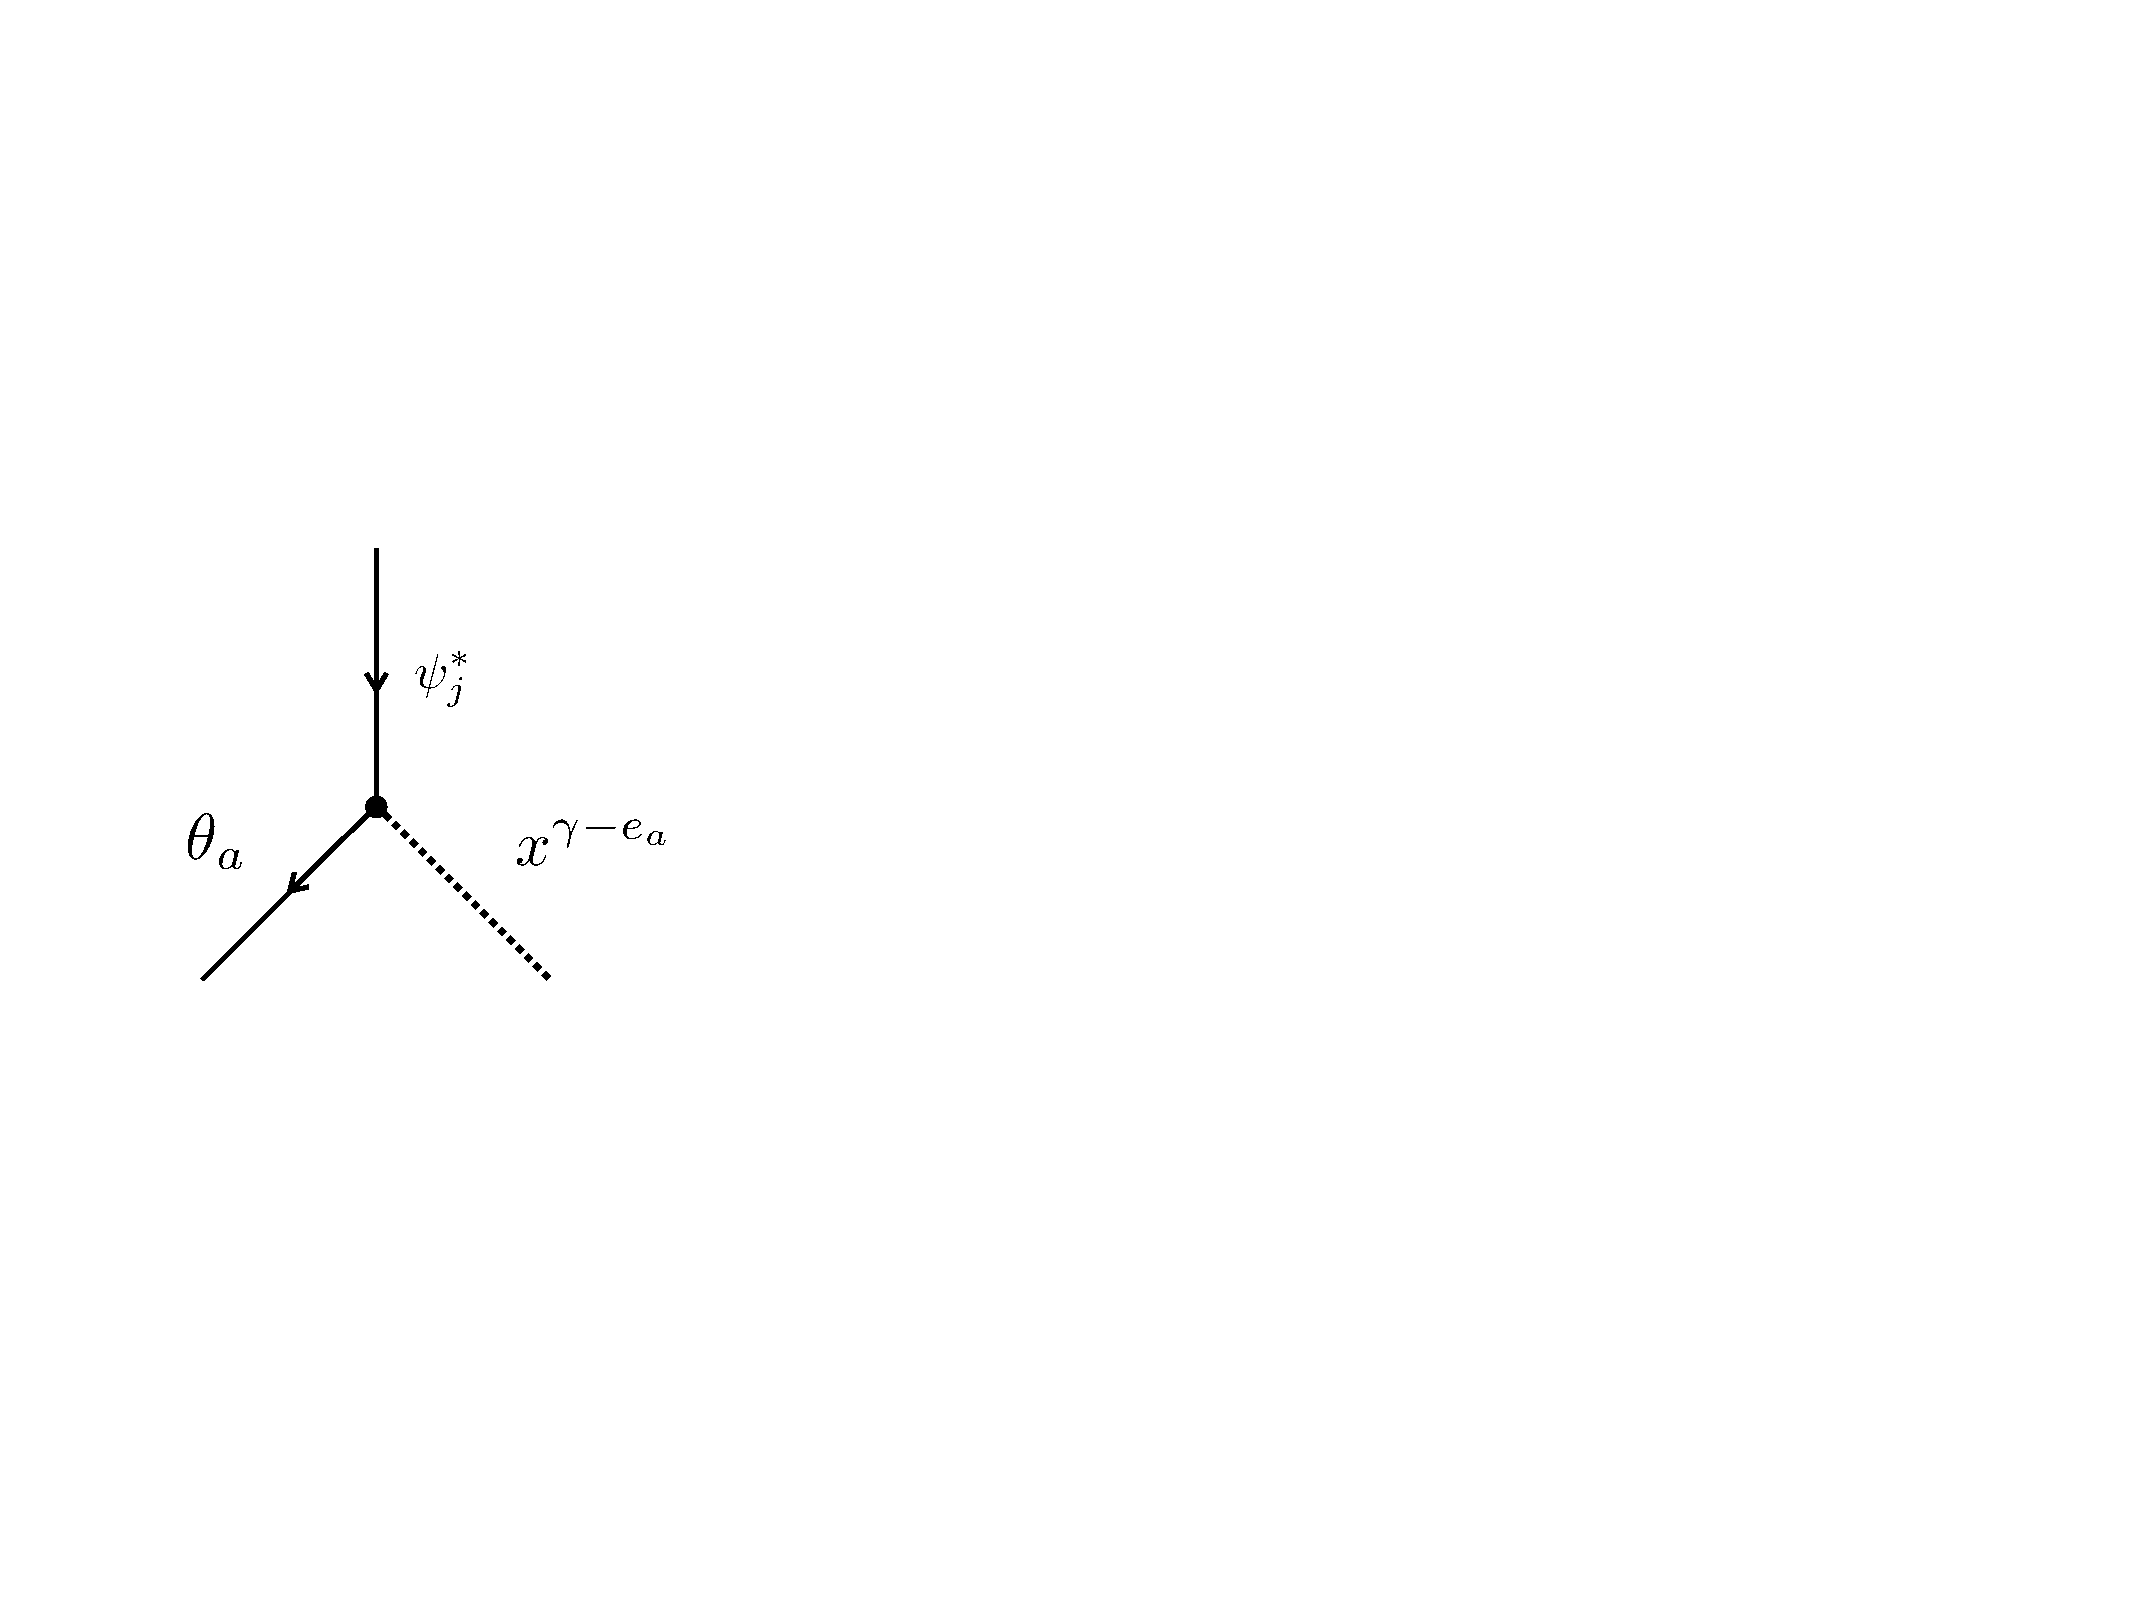
\includegraphics[scale=0.4]{dia2}
&
$\theta_a x^{\gamma - e_a} \big[\psi_j, -\big] \in \End_k( \mathscr{H} )$\\
\vspace{0.5cm}
$1 \le a,j \le n\,, \gamma \in \mathbb{N}^n$
&
\tagarray{\label{interaction_1}}
\end{tabular}
\end{center}

\begin{center}
\begin{tabular}{ >{\centering}m{1cm} >{\centering}m{4cm} >{\centering}m{8cm} >{\centering}m{1cm}}
\textbf{B}
&
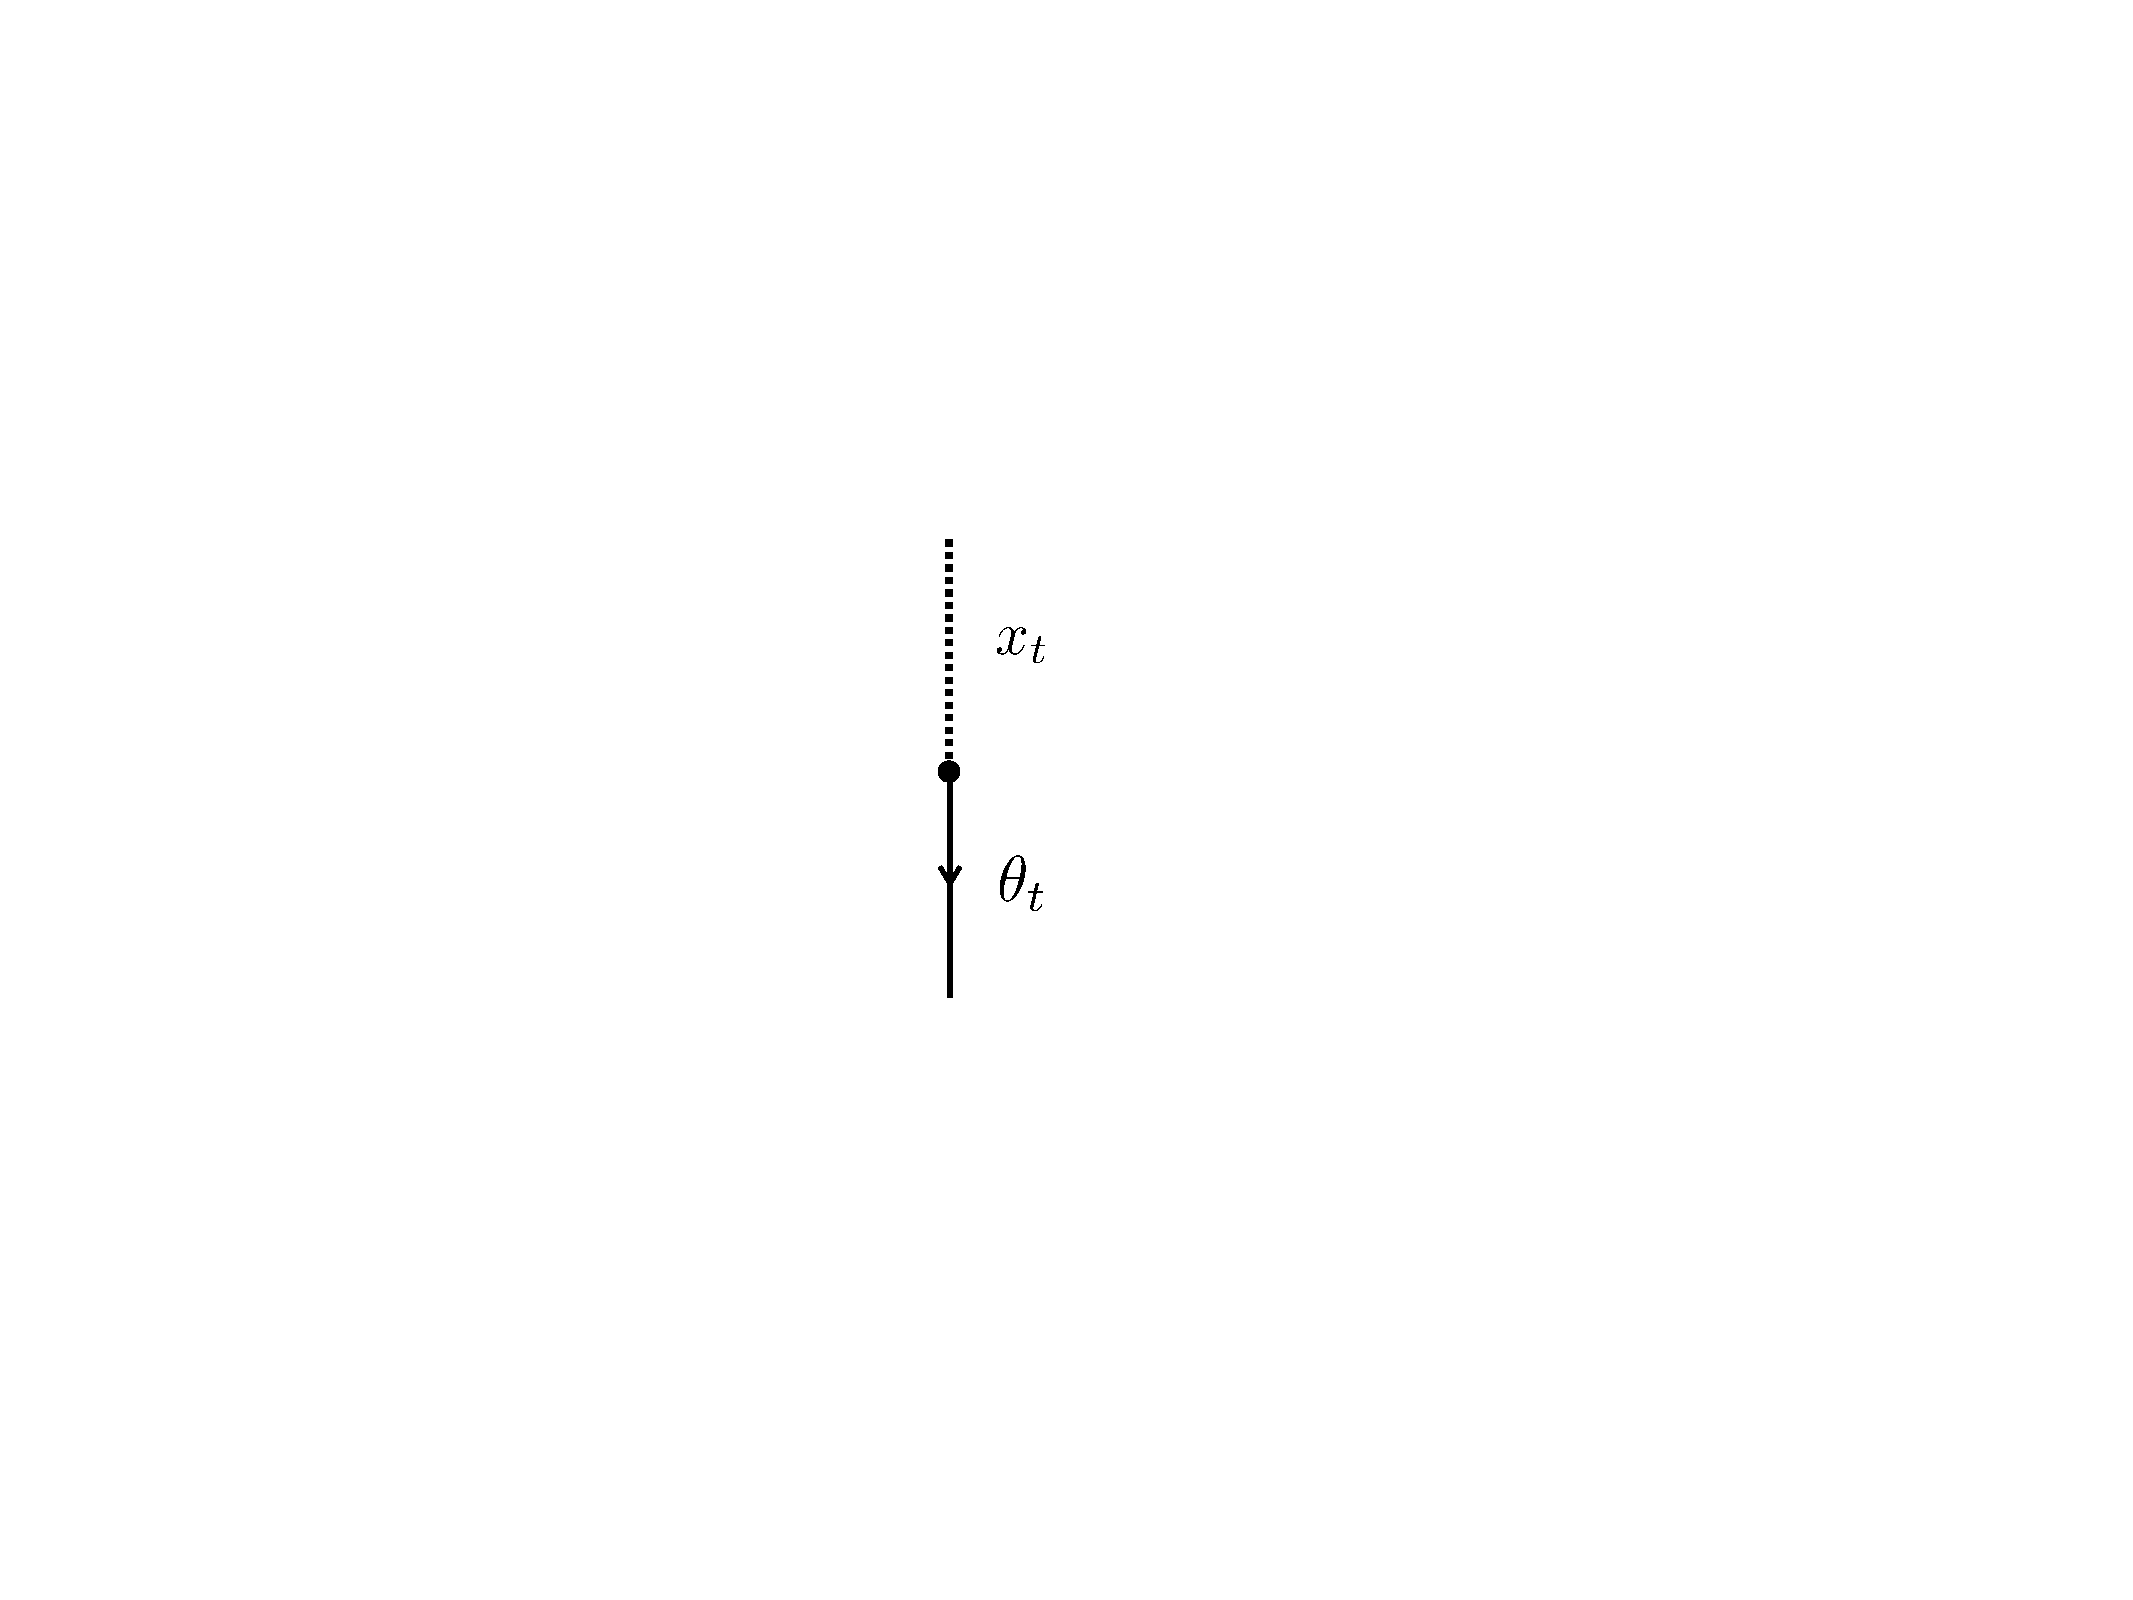
\includegraphics[scale=0.4]{dia3}
&
$\theta_t \partial_t \in \End_k( \mathscr{H} )$\\
\vspace{0.5cm}
$1 \le t \le n$
&
\tagarray{\label{interaction_2}}
\end{tabular}
\end{center}

\begin{center}
\begin{tabular}{ >{\centering}m{1cm} >{\centering}m{4cm} >{\centering}m{8cm} >{\centering}m{1cm}}
\textbf{C}
&
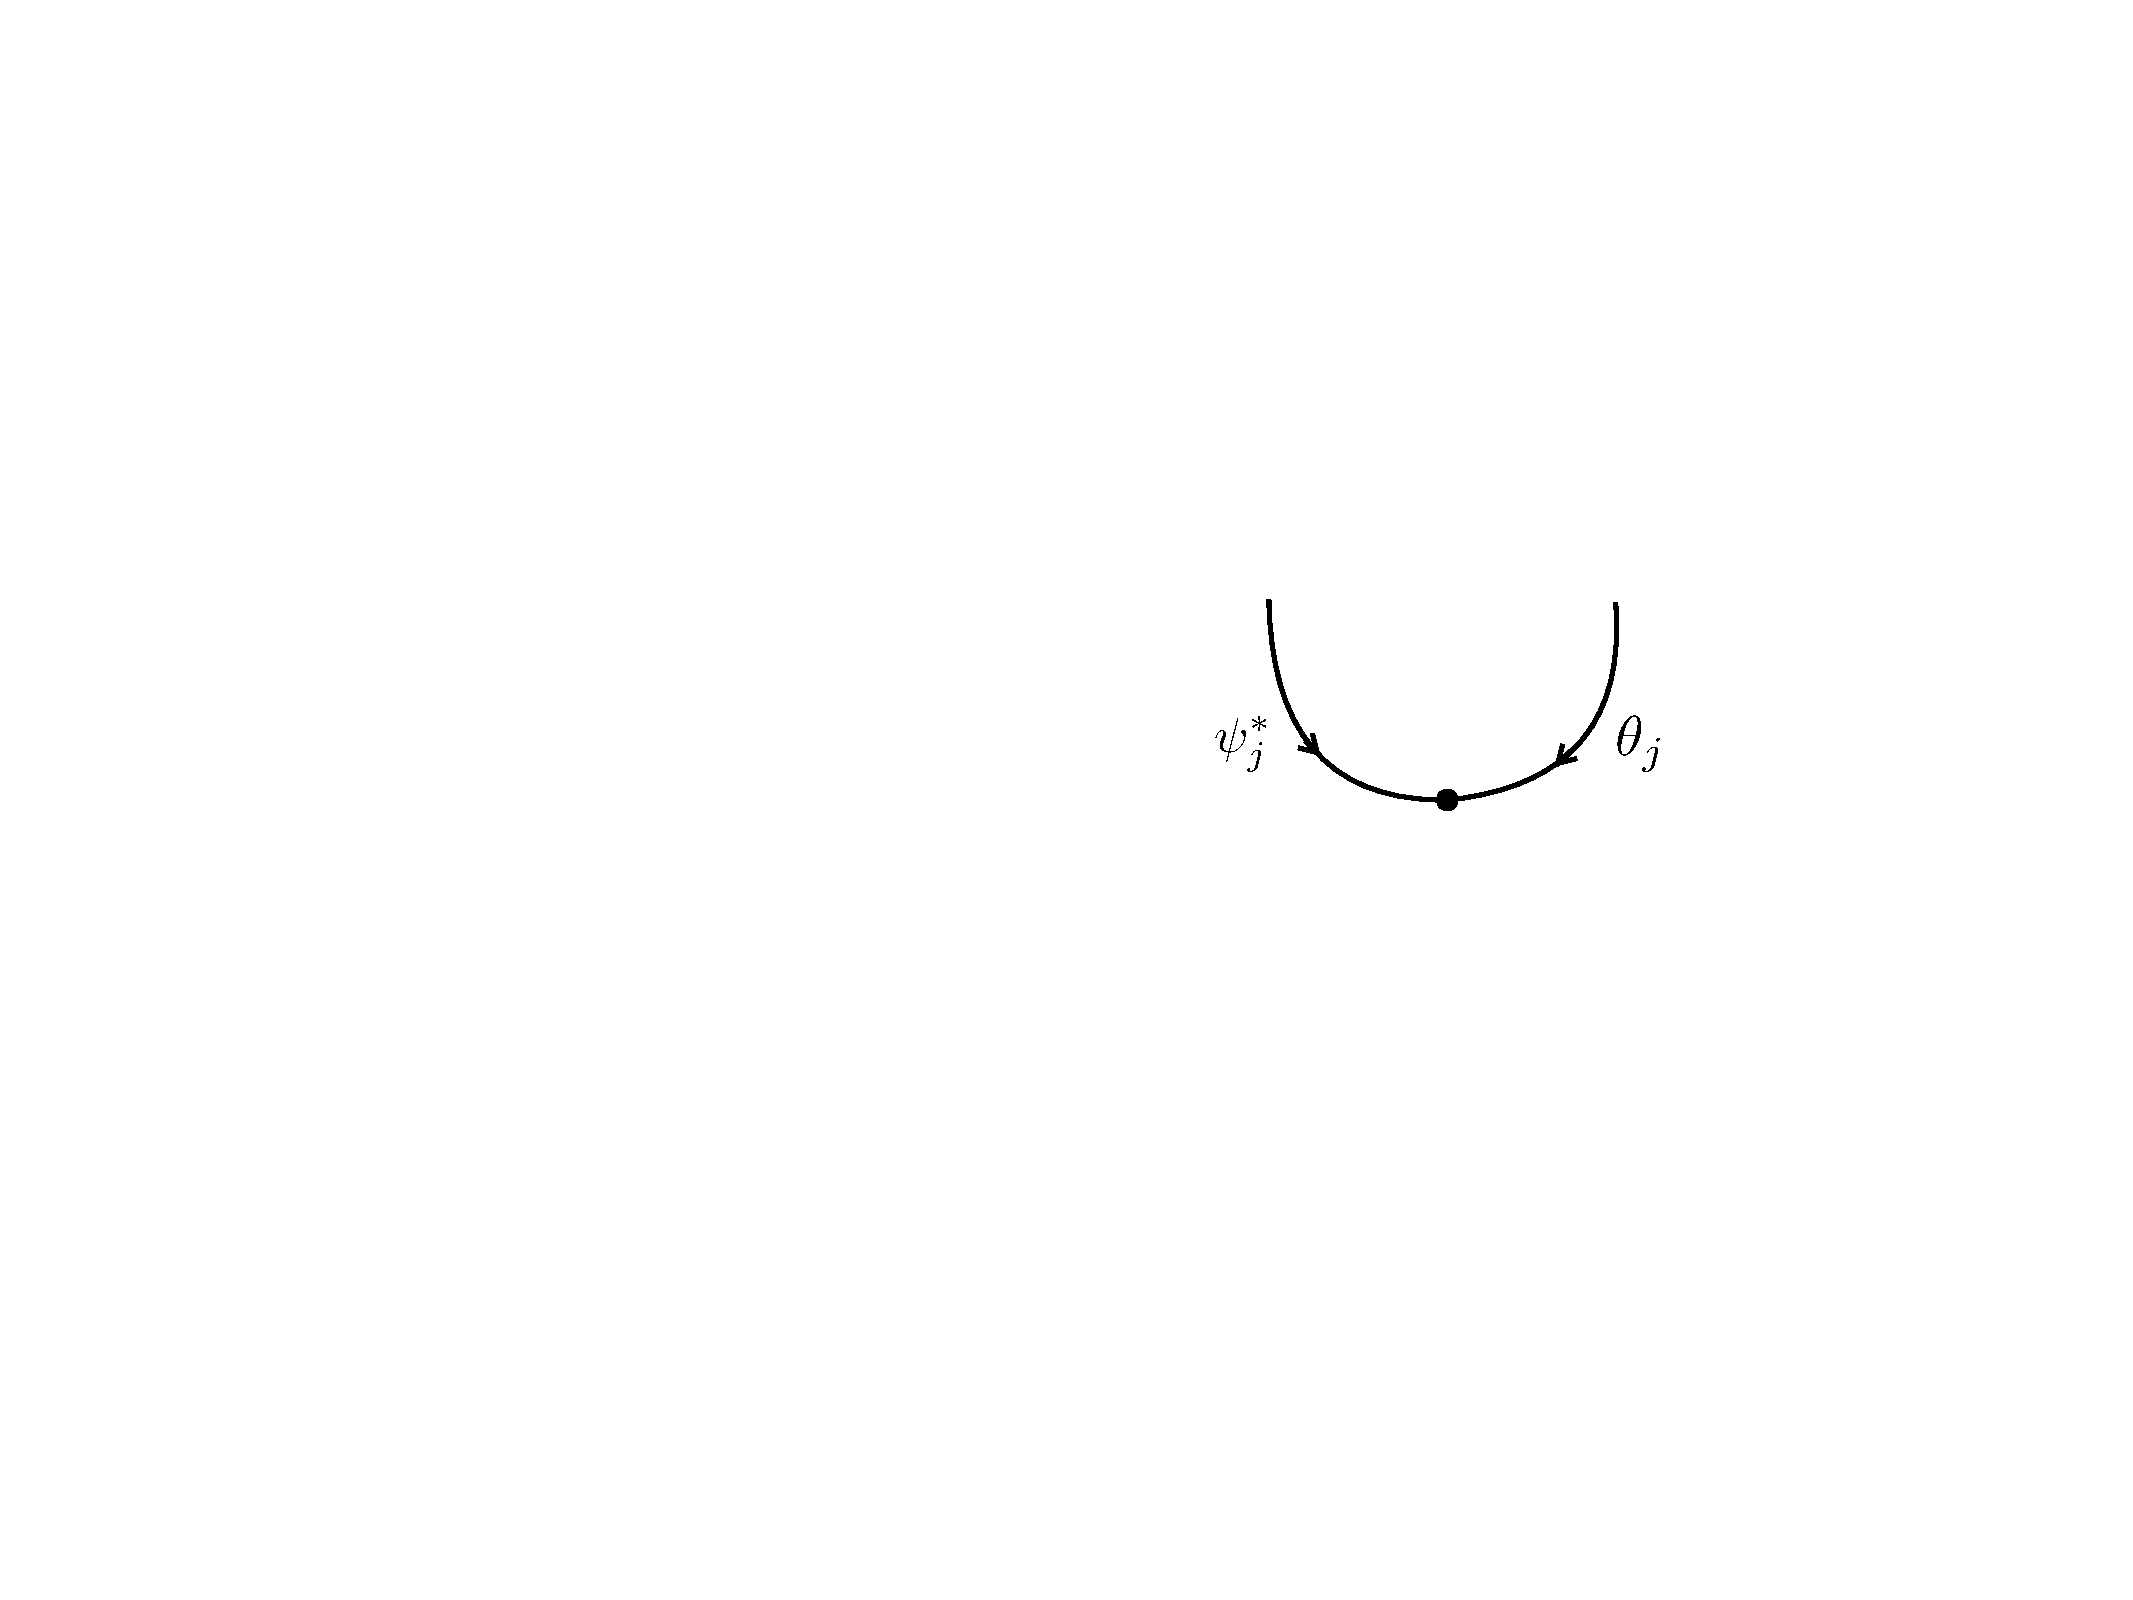
\includegraphics[scale=0.4]{dia4}
&
$m_2 \big( \big[\psi_j,-\big] \otimes \theta_j^* \big) \in \Hom_k( \mathscr{H}^{\otimes 2}, \mathscr{H} )$\\
\vspace{0.5cm}
$1 \le j \le n$
&
\tagarray{\label{interaction_3}}
\end{tabular}
\end{center}
Here $m_2$ is the multiplication in $\mathscr{H}$ and, given $\gamma \in \mathbb{N}^n$, we write $x^\gamma = x_1^{\gamma_1} \cdots x_n^{\gamma_n}$, with $e_i \in \mathbb{N}^n$ the unit vector with $x^{e_i} = x_i$. By convention if $\gamma_a = 0$ then $x^{\gamma - e_a} = 0$. Finally, note that in the Feynman diagrams, bosonic particles are depicted with dotted lines, and fermionic particles with solid lines.

These interactions ``take place'' at vertices of the tree $A(T)$ for some $T \in \cat{T}_q$, and come with the following constraints, which will be formalised below in terms of combinatorial data called \emph{configurations}. We write $f(\gamma)$ for the coefficient of $x^\gamma$ in a polynomial $f \in R$ and recall the chosen decomposition $W = \sum_j x_j W^j$. 

\begin{itemize}
\item A-type interactions only occur at input vertices and internal edges of $T$.
\item B-type interactions only occur at internal edges of $T$, and moreover there is \emph{precisely one} at each internal edge.
\item C-type interactions only occur at internal vertices of $T$.
\item The A-type interaction with indices $a,j, \gamma$ appears with the coefficient
\be\label{eq:coeff_a}
-\frac{\gamma_a}{|\gamma|} W^j( \gamma)
\ee
where $|\gamma| = \sum_i \gamma_i$. Each B- and C-type interaction appears with coefficient $(-1)$.
\end{itemize}

As we will see, the coefficient \eqref{eq:coeff_a} is the only way that $W$ enters the rules, and thus the definition of the $A_\infty$-products on $\mathscr{B}$. The precise definition of the Feynman rules will be given in Definition \ref{defn:config} below, but first we give an example of a tree with interactions inserted, to illustrate the various ingredients.

\begin{example} Consider the tree $T \in \cat{T}_3$ whose augmented tree $A(T)$ is depicted below, together with labels for its vertices, where we label by $e$ the vertex corresponding to the internal edge of $T$:
\begin{center}
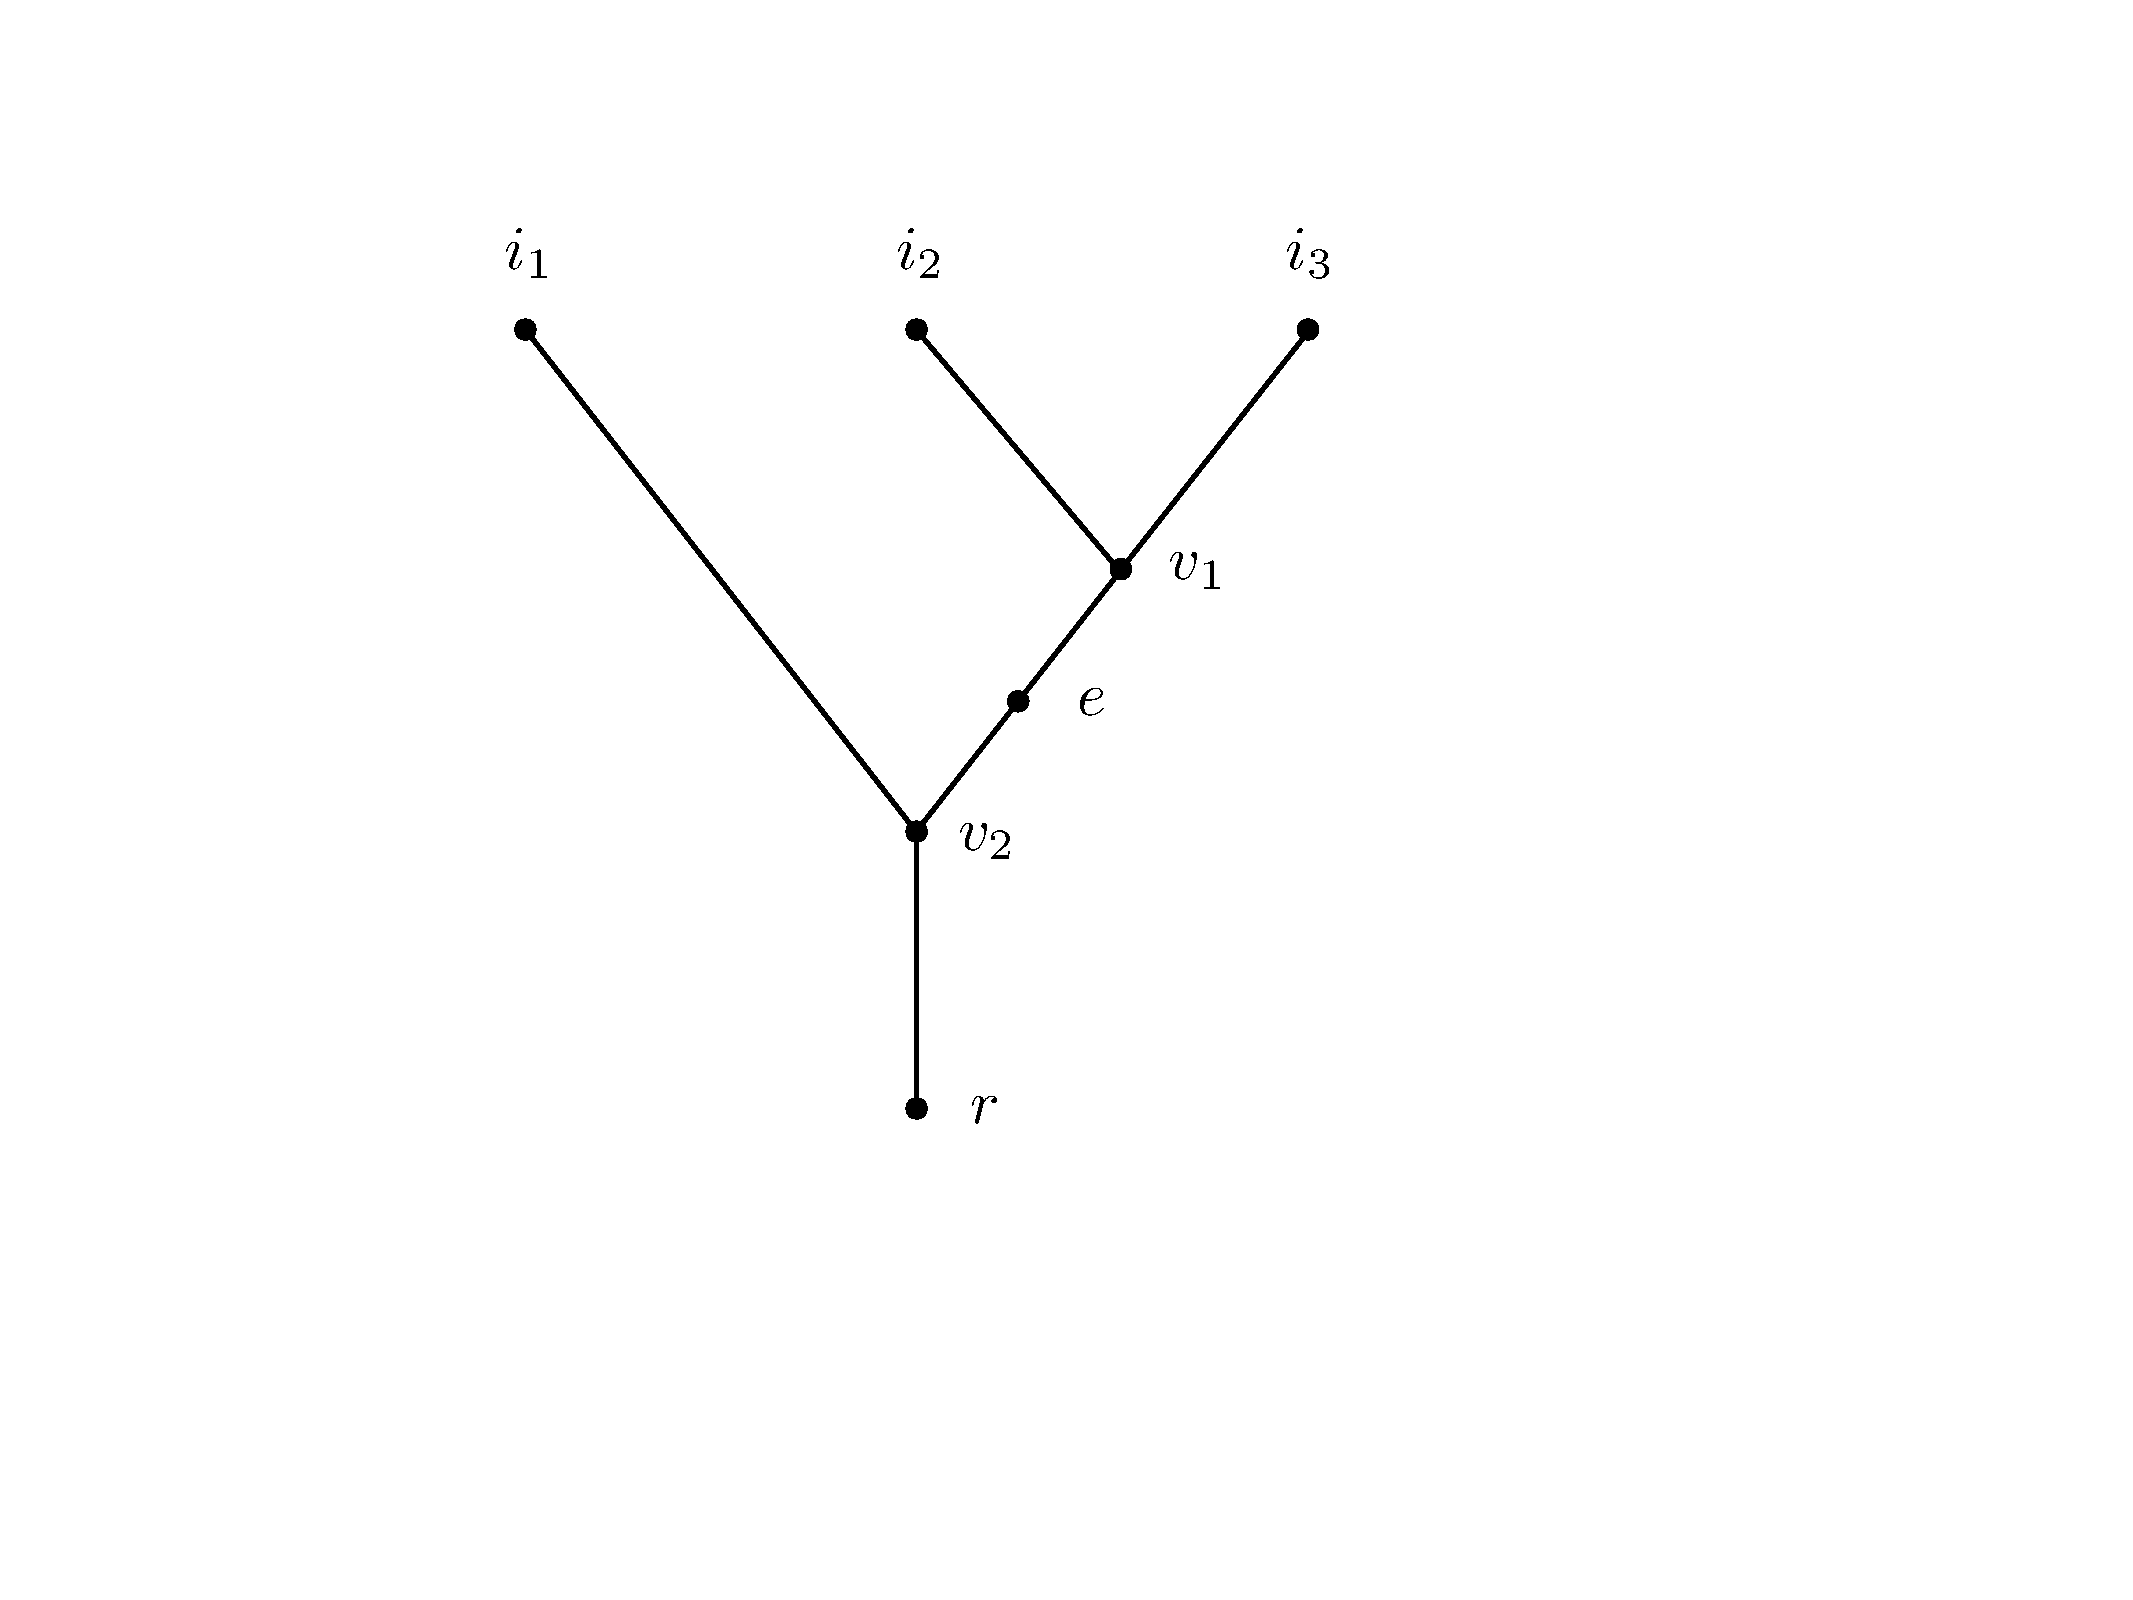
\includegraphics[scale=0.25]{dia7}
\end{center}
Set $W = x^3 \in \mathbb{C}[x]$ so that $W^1 = x^2$ and the only A-type interaction has $a = 1, j = 1, \gamma = 2$ and coefficient $1$, as in the diagram (we write $\theta = \theta_1, \psi = \psi_1$)
\begin{center}
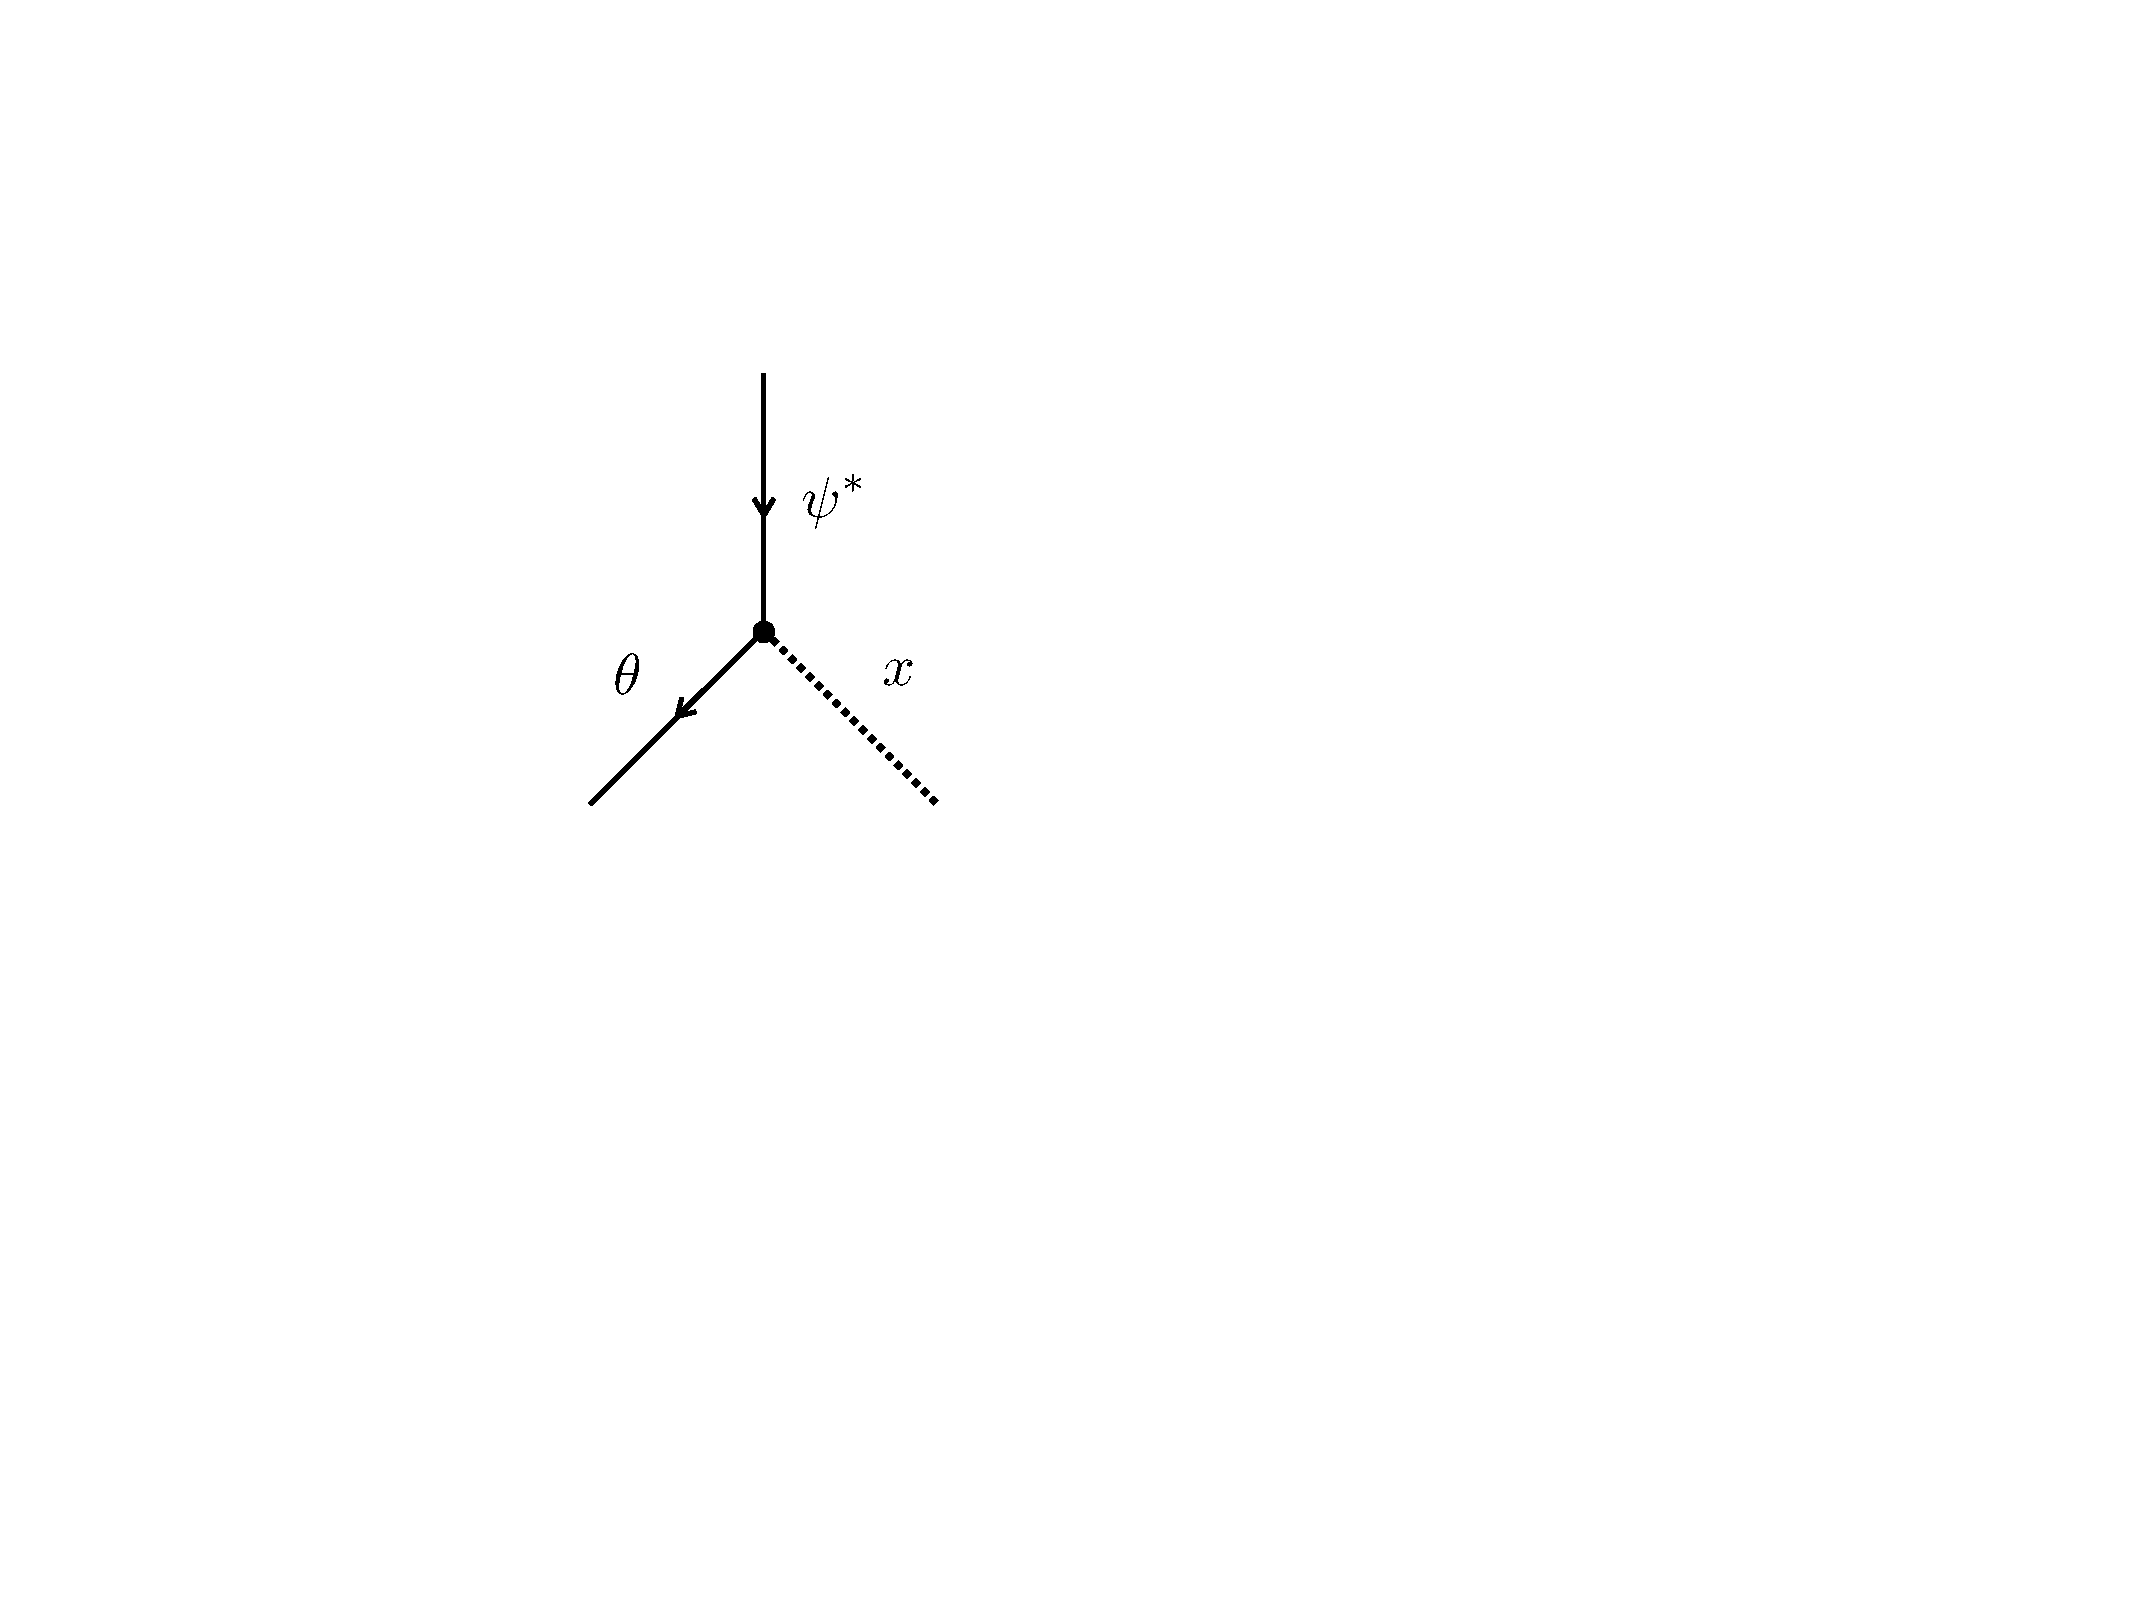
\includegraphics[scale=0.3]{dia5}
\end{center}
Consider the input state $\Psi = \psi^* \otimes \psi^* \otimes \psi^*$ in $\mathscr{B}^{\otimes 3}$. One possible pattern of interactions (called a configuration, below) has a single A-type interaction at the input vertex $i_3$, a B-type interaction at $e$, and two C-type interactions at $v_1,v_2$, as shown in
\begin{center}
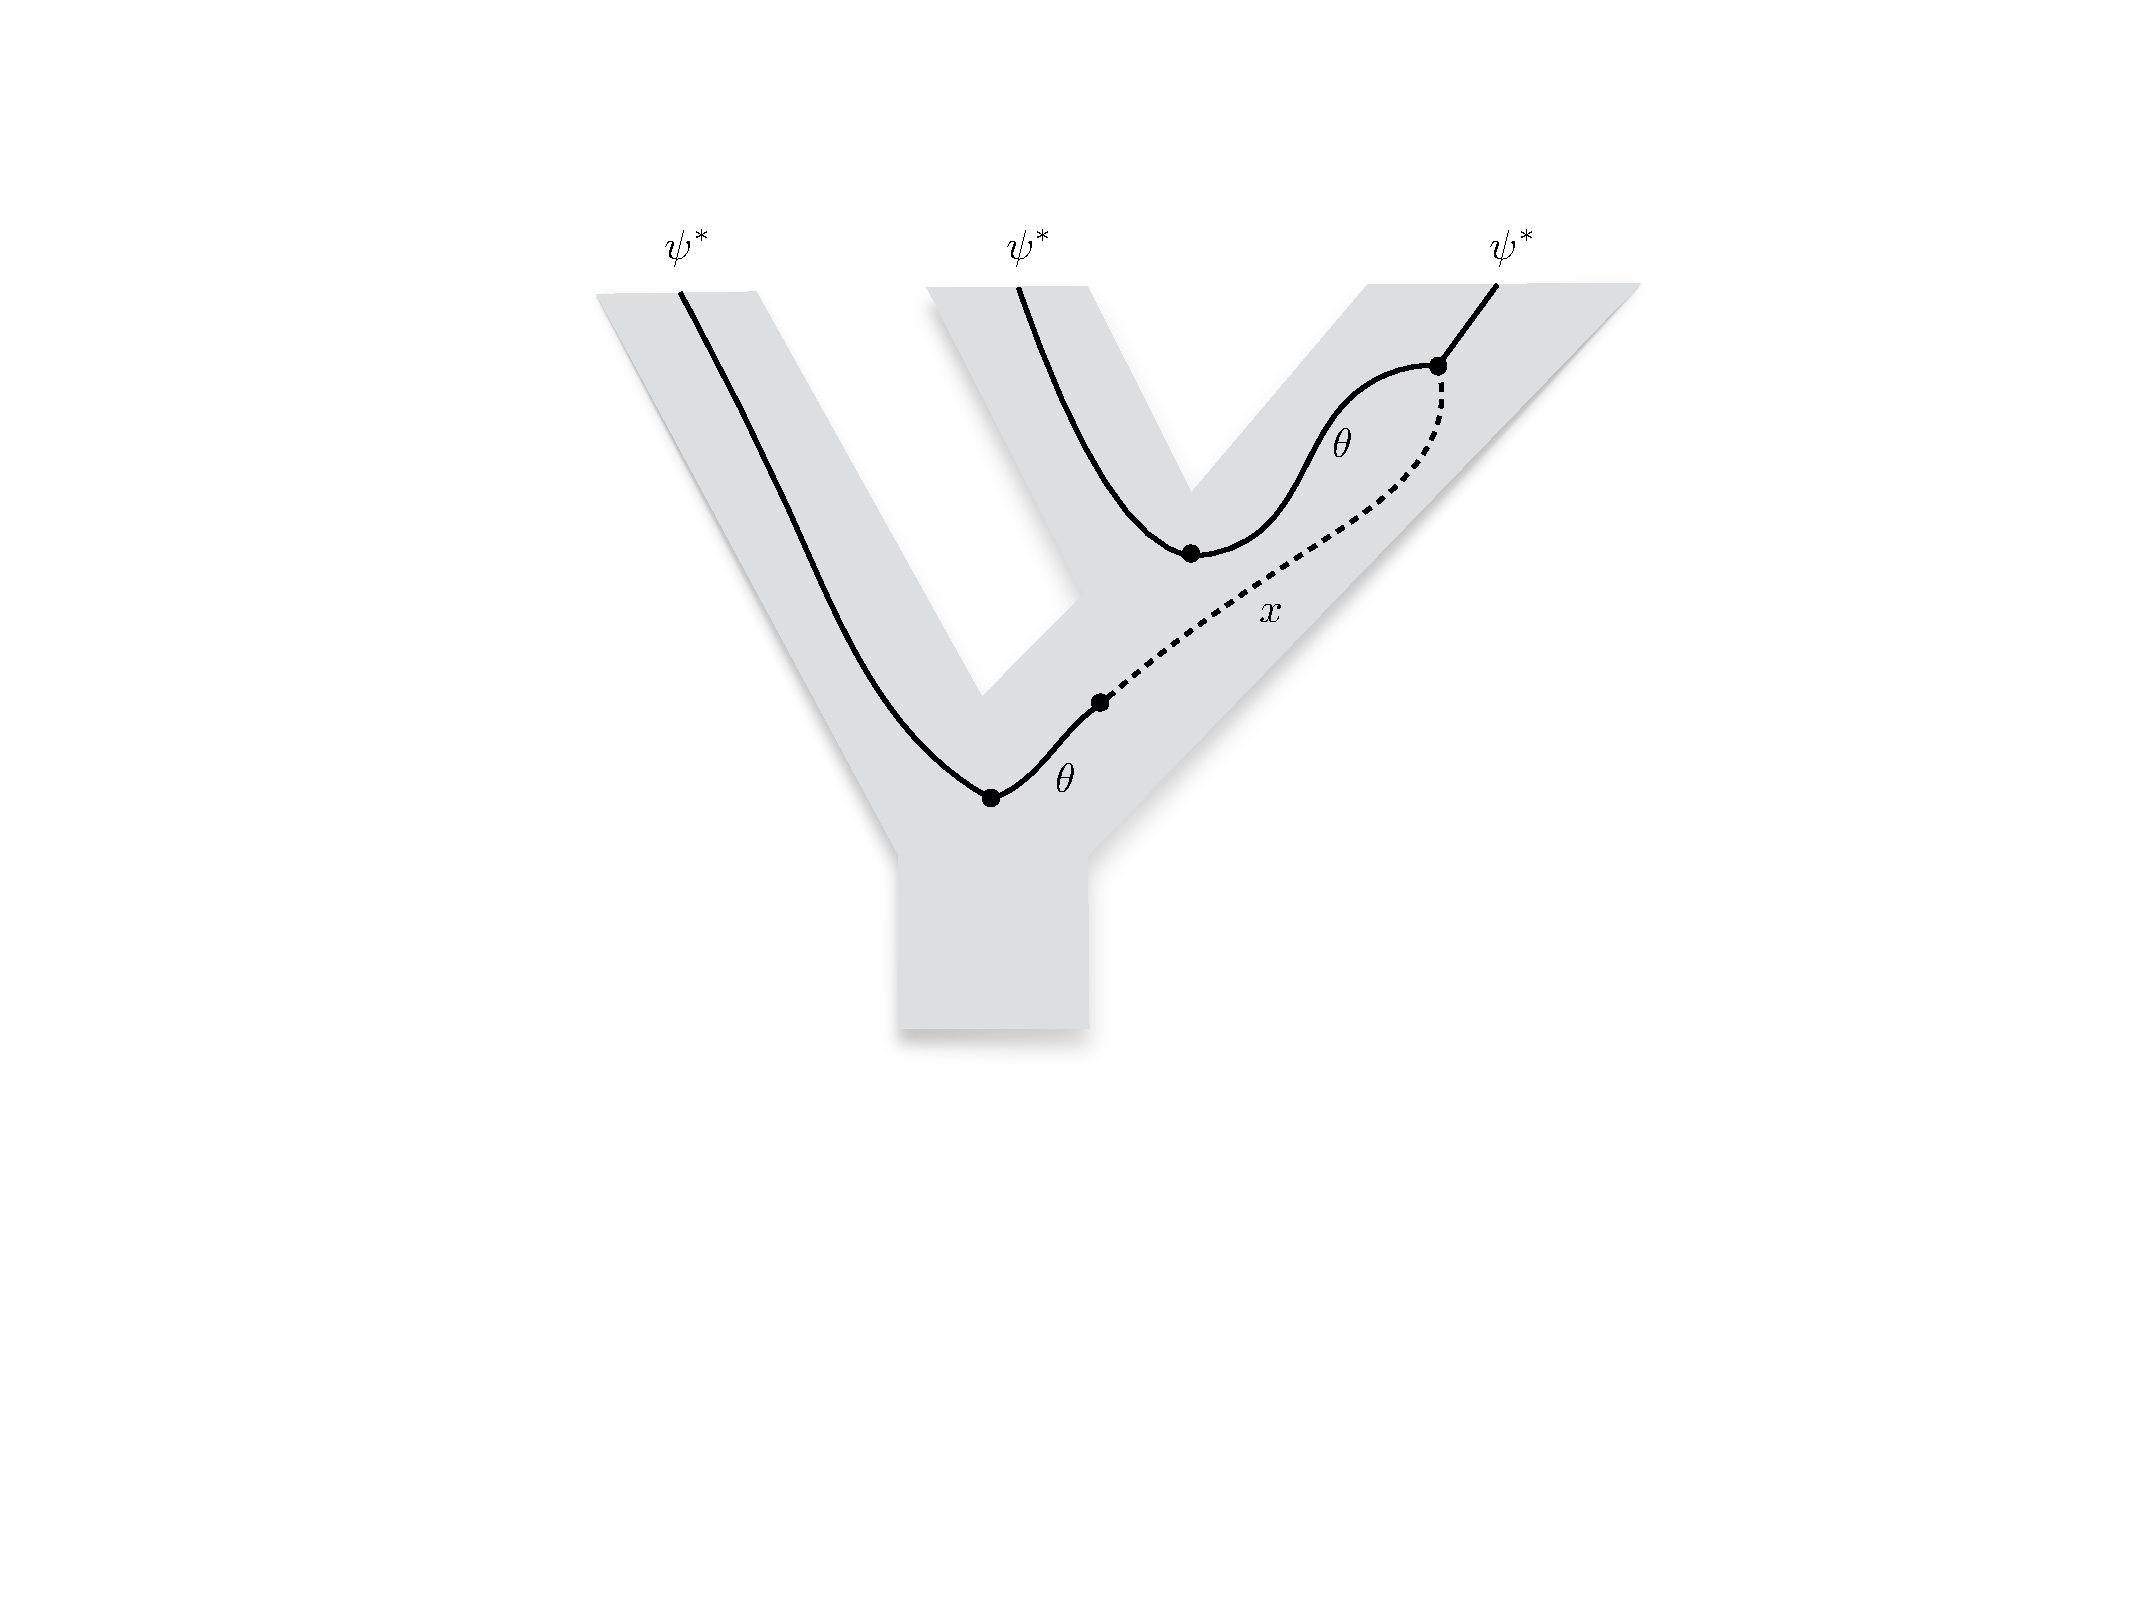
\includegraphics[scale=0.3]{dia6}
\end{center}
This ``topological'' Feynman diagram depicts the value of the linear map
\begin{align*}
(-1)^3 p \circ m_2 \big([\psi, -] \otimes \theta^*\big) \circ \big( \iota \otimes \theta \partial_x \circ m_2 ([\psi, -] \otimes \theta^*)\big( \iota \otimes \theta x [\psi, -] \iota \big)\big)
\end{align*}
on the input state $\Psi$, which may be checked is $-1 \in \mathscr{B}$.
\end{example}

Now we give a precise definition of the Feynman rules. Let $T \in \cat{T}_q$ be a valid plane tree with $q$ inputs and $e_i(T)$ internal edges, and let $A(T)$ be the augmented plane tree. 

\begin{definition}\label{defn:config} A \emph{configuration} $C$ of a valid plane tree $T$ consists of the following data, for each non-root vertex $v$ of $A(T)$:
\begin{itemize}
\item An integer $m(v) \ge 0$.
\item A subset $J(v) \subseteq \{ 1,\ldots, n \}$ with $|J(v)| = m(v)$. 
\item If $v$ is an input, or comes from an internal edge of $T$, a pair
\[
( a_j(v), \gamma_j(v) ) \in \{ 1, \ldots, n \} \times \mathbb{N}^n
\]
for each $j \in J(v)$.
\item If $v$ comes from an internal edge of $T$, an integer $t(v) \in \{1,\ldots,n\}$.
\end{itemize}
Let $\operatorname{Con}(T)$ denote the set of all configurations.
\end{definition} 

\begin{remark} The integer $m(v)$ counts \emph{how many} interactions take place at $v$. The set $J(v)$ consists of all $j$-indices appearing in interactions at $v$. The interactions of A-type (at inputs and internal edges) are defined by indices $a_j(v), \gamma_j(v)$ while at each internal edge $e$ of $T$, $t(e)$ is the index of the C-type interaction.
\end{remark}

\begin{definition} Given a tree $T \in \cat{T}_q$ and configuration $C \in \operatorname{Con}(T)$ we define a decoration $D_{T,C}$ of $A(T)$ by the assignment of the modules
\begin{itemize}
\item $\mathscr{B}$ to the input at each non-root leaf and the output at the root, and
\item $\mathscr{H}$ to each edge.
\end{itemize}
To each vertex $v$ of $A(T)$ we associate an operator $\phi_v$ as follows, writing $m, J, \{ (a_j, \gamma_j) \}_{j \in J}, t$ for the data associated to $v$ by the configuration $C$:
\begin{itemize}
\item if $v$ is an input, then $\phi_v$ is the linear map $\mathscr{B} \lto \mathscr{H}$ given by
\be\label{eq:int_input}
\phi_v = (-1)^m \prod_{j \in J}\Big\{ \frac{(\gamma_j)_a}{|\gamma_j|} W^j( \gamma_j)  \theta_{a_j} x^{\gamma_j - e_{a_j}} \big[ \psi_j, - \big] \Big\} \circ \iota\,.
\ee
Note that the operator under the product is even, so the order is irrelevant.
\item if $v$ comes from an internal edge of $T$, then
\be\label{eq:int_intedge}
\phi_v = (-1)^m \prod_{j \in J} \Big\{ \frac{(\gamma_j)_a}{|\gamma_j|} W^j( \gamma_j)  \theta_{a_j} x^{\gamma_j - e_{a_j}} \big[ \psi_j, - \big] \Big\} \circ \theta_t \partial_t\,.
\ee
\item if $v$ comes from an internal vertex of $T$, then
\be\label{eq:int_intvert}
\phi_v = (-1)^m m_2 \circ \prod_{j \in J} \Big\{ \big[ \psi_j, - \big] \otimes \theta_j^* \Big\}
\ee
which is a map $\mathscr{H}^{\otimes 2} \lto \mathscr{H}$. Here $m_2$ denotes the product on $\mathscr{H}$.
\item if $v = r$ is the root, $\phi_v = p: \mathscr{H} \lto \mathscr{B}$ is the projection defined in \eqref{??}.
\end{itemize}
\end{definition}

Finally, there is a symmetry factor.

\begin{definition} Given a sequence $a_1,\ldots,a_m \ge 1$ of integers and $a \ge 0$ we define
\begin{align*}
\tau(a, a_1, \ldots, a_m) &= a_1 \cdots a_m \sum_{\sigma \in \mathfrak{S}_m} \prod_{i=0}^{m-1} \frac{1}{a + \sum_{j=m-i}^m a_{\sigma(j)}}\\
&= a_1 \cdots a_m \sum_{\sigma \in \mathfrak{S}_m} \frac{1}{a + a_{\sigma(m)}} \cdots \frac{1}{a + a_{\sigma(1)} + \cdots + a_{\sigma(m)}}\,.
\end{align*}
\end{definition}

\begin{definition} Given $T \in \cat{T}_q, C \in \operatorname{Con}(T)$ and an internal edge $e$ of $T$ we define
\[
\omega(C, e) = \sum_{e' < e} \sum_{j \in J(e')} | \gamma_j(e') | - \sum_{z < e} m(z)
\]
where the sum is over all internal edges and input vertices $e'$ above $e$ in $A(T)$ i.e. for each $e$ is on the unique path from $e'$ to the root, and $z$ ranges over internal vertices. 

We define in addition a symmetry factor
\begin{gather*}
S(C, e) = \frac{1}{\omega(C,e)} \tau\big( \omega(C,e), \{ |\gamma_j(e)| \}_{j \in J(e)} \big) \in \mathbb{Q}\,,\\
S(C) = \prod_{e \in E_i(T)} S(C,e)
\end{gather*}
where $E_i(T)$ is the set of internal edges $e$ of $T$.
\end{definition}

\begin{definition} Given $T \in \cat{T}_q$ and $C \in \operatorname{Con}(T)$ we define the $k$-linear operator
\[
\cat{O}(T, C): \mathscr{B}^{\otimes q} \lto \mathscr{B}
\]
to be the denotation $\cat{O}(T,C) = \langle D_{T,C} \rangle$, defined without Koszul signs.
\end{definition}

\begin{definition} We define $\rho_q: \mathscr{B}[1]^{\otimes q} \lto \mathscr{B}[1]$ by
\[
\rho_q( \Lambda_1 \otimes \cdots \otimes \Lambda_q ) = \sum_{T \in \cat{T}_q} \sum_{C \in \operatorname{Con}(T)} (-1)^{Q(T, \underline{\Lambda})} S(C) \cdot \cat{O}(T, C)( \Lambda_q \otimes \cdots \otimes \Lambda_1 )\,.
\]
where
\[
Q(T, \underline{\Lambda}) = sign\,.
\]
\end{definition}

\begin{theorem} The operators $\rho_q$ satisfy the forward suspended $A_\infty$-constraints, so that $(\mathscr{B}, \{ \rho_q \}_{q \ge 2})$ is an $A_\infty$-algebra, and it is quasi-isomorphic to $\End_k(k^{\stab})$.
\end{theorem}

\section{The minimal model}

We define the even operator $\delta_i = \psi_i \theta_i^*$ on the underlying module $\eqref{eq:same_underlying}$ of $S \otimes \md{A}_W$, so that $\delta = \sum_i \delta_i$. Since $[ \delta_i, \delta_j ] = 0$ for all $i,j$ we have
\be
\exp(\pm \delta) = \exp(\pm \delta_1) \cdots \exp(\pm \delta_n)\,.
\ee

\begin{lemma} For $1 \le i \le n$ there is a commutative diagram
\be
\xymatrix@C+3pc@R+1pc{
(S \otimes \md{A}_W) \otimes (S \otimes \md{A}_W) \ar[d]_-{\delta_i \otimes 1 + 1 \otimes \delta_i + [\psi_i,-] \otimes \theta_i^*} \ar[r]^-{m_2} & S \otimes \md{A}_W \ar[d]^-{\delta_i}\\
(S \otimes \md{A}_W) \otimes (S \otimes \md{A}_W) \ar[r]_-{m_2} & S \otimes \md{A}_W
}
\ee
\end{lemma}

\begin{definition} We define
\be
\Xi_i = [ \psi_i, - ] \otimes \theta_i^* : S \otimes \md{A}_W \lto S \otimes \md{A}_W\,.
\ee
and
\be
\Xi = \sum_i \Xi_i\,.
\ee
\end{definition}

\begin{proposition} There is a commutative diagram
\be
\xymatrix@C+3pc@R+2pc{
(S \otimes \md{A}_W) \otimes (S \otimes \md{A}_W) \ar[d]_-{\exp(-\delta) \otimes \exp(-\delta)} \ar[r]^-{m_2} & S \otimes \md{A}_W \ar[dd]^-{\exp(-\delta)}\\
(S \otimes \md{A}_W) \otimes (S \otimes \md{A}_W) \ar[d]_-{\exp(-\Xi)}\\
(S \otimes \md{A}_W) \otimes (S \otimes \md{A}_W) \ar[r]_-{m_2} & S \otimes \md{A}_W
}
\ee
\end{proposition}

\bibliographystyle{amsalpha}
\providecommand{\bysame}{\leavevmode\hbox to3em{\hrulefill}\thinspace}
\providecommand{\href}[2]{#2}
\begin{thebibliography}{BHLS03}
  
  \bibitem[Dyc11]{d0904.4713}
T.~Dyckerhoff, \textsl{Compact generators in categories of matrix factorizations},
  Duke Math. J. \textbf{159} (2011), 223--274,
  \href{http://arxiv.org/abs/0904.4713}{[arXiv:0904.4713]}.
  
\bibitem{lazaroiu}
C.~I.~Lazaroiu, \textsl{Generating the superpotential on a D-brane category: I}, [arXiv:hep-th/0610120].
  
\bibitem{murfet}
D.~Murfet, \textsl{Computing with cut systems}, \href{http://arxiv.org/abs/1402.4541}{[arXiv:1402.4541]}.

\bibitem{lgdual}
N.~Carqueville and D.~Murfet, \textsl{Adjunctions and defects in Landau-Ginzburg models}, Adv. Math. \textbf{289} (2016), 480--566.

\bibitem{dm1102.2957}
T.~Dyckerhoff and D.~Murfet, \textsl{Pushing forward matrix factorisations}, Duke Math. J. \textbf{162} (2013), 1249--1311.

\end{thebibliography}

\end{document}